\section*{Metodología}
La metodología implementada comprende: (i) adquisición de datos base, (ii) limpieza y preprocesamiento con umbrales y reglas reproducibles, (iii) enriquecimiento geoespacial mediante capas del distrito y conteos de POIs (OSM), (iv) entrenamiento y evaluación de modelos base y aumentados, y (v) persistencia y exposición vía API.

\begin{figure}[h]
    \centering
    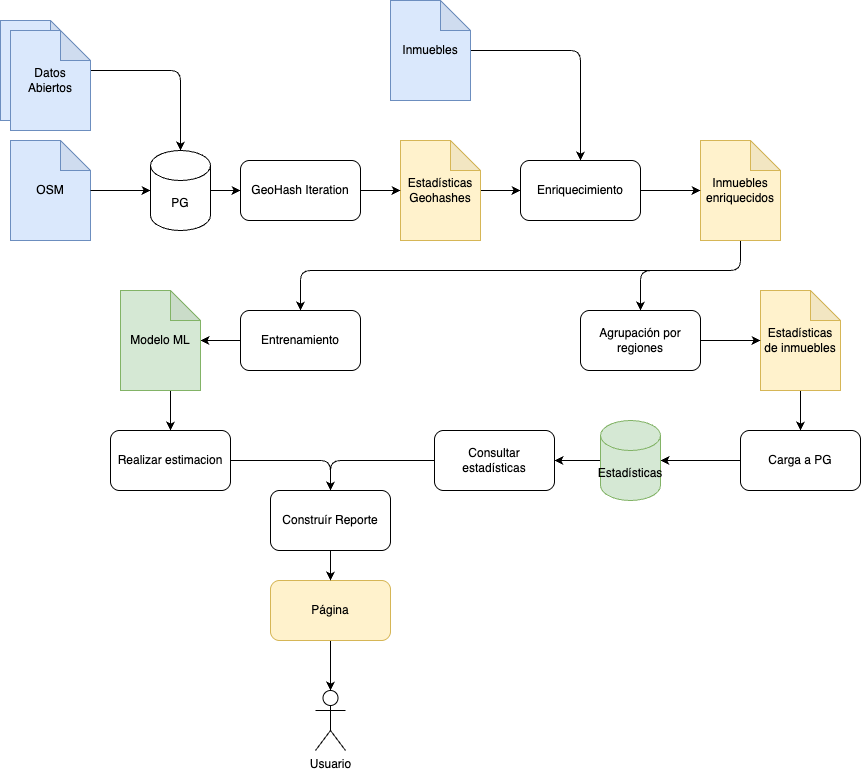
\includegraphics[width=0.85\linewidth]{Images/metodologia.png}
    \caption{Proceso general de la metodología}
    \label{fig:metodologia}
\end{figure}

\subsection*{Fuentes de datos}
\begin{itemize}
    \item \textbf{Datos de inmuebles (base)}: JSON único de agosto de 2024 publicado en GitHub (\texttt{builker-col/bogota-apartments}). Se procesó a CSV.
    \item \textbf{Datos abiertos del distrito (PostGIS)}: capas consultadas en agosto de 2025: \texttt{barrios\_bogota}, \texttt{upz\_bogota}, \texttt{localidades\_bogota}, \texttt{estratos\_manzana}, \texttt{avaluo\_catastral\_manzana}, y POIs OSM (\texttt{gis\_osm\_pois\_free\_1}, \texttt{gis\_osm\_pois\_a\_free\_1}), con SRID esperado 4326.
\end{itemize}

\subsection*{Limpieza y preprocesamiento}
Realizado en Python (\textit{Pandas}, \textit{NumPy}, \textit{scikit-learn}) sobre el CSV base:
\begin{itemize}
    \item \textbf{Outliers}: filtro por percentil 99. \emph{Área} \(\leq 464\,m^2\), \emph{precio\_venta} \(\leq 5{,}4\times 10^9\) COP.
    \item \textbf{Precio mínimo}: \(\geq 50{,}000{,}000\) COP.
    \item \textbf{Área igual a 0}: imputación por mediana de comparables (mismo \emph{estrato}, \emph{habitaciones}, \emph{banos}, \emph{sector}); si no hay, mediana por \emph{estrato}.
    \item \textbf{Parqueaderos negativos}: reemplazo por moda dentro del mismo \emph{estrato} (sino, moda global).
    \item \textbf{Coordenadas}: imputación por mediana del \emph{sector} o global cuando estén fuera de Bogotá; bounding box final: lat \([4.4, 4.9]\), lon \([-74.3, -73.9]\). Registros fuera se eliminan tras imputación.
    \item \textbf{Estrato fuera de rango [1--6]}: imputación por modo del \emph{sector}; si no hay, modo global.
\end{itemize}

\subsection*{Enriquecimiento geoespacial}
Se calcula por propiedad (lat, lon) con un pipeline asíncrono y persistencia en PostGIS:
\begin{itemize}
    \item \textbf{Conteos de POIs OSM} por radios de 100, 300, 500, 1000 y 2000 metros en categorías agregadas: \emph{education}, \emph{healthcare}, \emph{retail\_access}, \emph{dining\_and\_entertainment}, \emph{accommodation}, \emph{parks\_and\_recreation}, \emph{infrastructure\_services}, \emph{cultural\_amenities}.
    \item \textbf{Metadatos regionales}: asignación de UPZ, barrio y localidad; variables \emph{upz\_calculada}, \emph{barrio\_calculado}, \emph{localidad\_calculada}.
    \item \textbf{Valuación por geohash}: promedios de \emph{catastral} y \emph{comercial} por celda (geohash), usando \texttt{avaluo\_catastral\_manzana}.
    \item \textbf{Persistencia y estadísticas}: escritura en \texttt{property\_data} y agregación en \texttt{region\_stats} (barrio, UPZ, localidad) vía \texttt{ST\_Contains}, con \(n\), medias, desviaciones y cuartiles.
\end{itemize}

\subsection*{Modelos base}
Conjunto de modelos evaluados con validación cruzada \(KFold=5,\ \texttt{shuffle=True},\ \texttt{random\_state=42}\), métrica RMSE (escala real). Preprocesamiento: \texttt{SimpleImputer} (media/moda), \texttt{StandardScaler}, \texttt{OneHotEncoder}. Resultados (aprox.):
\begin{itemize}
    \item \textbf{Random Forest}: RMSE \(\approx\) 245M (CV); en\ hold-out (20\%): RMSE \(\approx\) 250.6M, MAE \(\approx\) 129.9M, R\textsuperscript{2} \(\approx\) 0.915.
    \item \textbf{XGBoost / LightGBM}: RMSE \(\approx\) 245--246M (CV).
    \item \textbf{Lineales}: \(\approx\) 348M; \textbf{SVR}: \(\approx\) 913M.
\end{itemize}
Se evaluó además con \(\log(\textit{precio\_venta})\) y \(\log(\textit{area})\), mejorando métricas en escala original.

\subsection*{Modelos con datos aumentados}
Se entrenaron variantes con variables enriquecidas y selección reducida:
\begin{itemize}
    \item \textbf{v0 (XGB)}: \(\log(\textit{area})\), one-hot; variables estructurales dominan; enriquecidas con aporte marginal.
    \item \textbf{v1 (XGB reducido + barrio\_top)}: hold-out RMSE \(\approx\) 254.66M, MAE \(\approx\) 136.54M, R\textsuperscript{2} \(\approx\) 0.9139. Modelo exportado como \texttt{xgboost\_model\_2.1.pkl}.
    \item \textbf{v2 (XGB con búsqueda aleatoria)}: mejores hiperparámetros: \(n\_\textit{estimators}=500\), \(\textit{max\_depth}=9\), \(\textit{learning\_rate}=0.05\), \(\textit{subsample}=0.8\), \(\textit{colsample\_bytree}=0.8\), \(\alpha=0\), \(\lambda=1\). Hold-out: RMSE \(\approx\) 233.49M, MAE \(\approx\) 121.96M, R\textsuperscript{2} \(\approx\) 0.9276. Exportado como \texttt{xgboost\_model\_2.2.pkl}.
\end{itemize}

\subsection*{Exposición de resultados y API}
Se expone un endpoint \texttt{GET /api/estimate} (FastAPI) que combina estadísticas del punto (POIs, región, valuación) y la predicción del modelo: agrega \texttt{get\_point\_stats}, \texttt{get\_region\_stats} y \texttt{estimate(...)} sobre la versión de modelo configurada (por defecto 2.1; se recomienda 2.2 por mejor RMSE).

\subsection*{Reproducibilidad}
Los notebooks en \texttt{analisis/notebooks/} contienen el detalle de extracción, limpieza, evaluación y entrenamiento; el proyecto \texttt{indexador-py/} encapsula el enriquecimiento y la persistencia en PostGIS. Se controlaron semillas aleatorias y configuración de validación para permitir replicación de métricas.

